\documentclass[letterpaper,11pt]{article}
\usepackage{jheppub}

\begin{document}

%%%%%%%%%%%%%%%%%%%%%%
\section*{Regularized likelihoods}
Author(s): Ioan-Mihail Dinu \\ \textit{Laboratoire de Phisique de Clermont, Clermont-Ferrand, France}\\

%\noindent \textit{Please do not write an introduction to anomaly detection - we will have one introduction at the beginning.  Furthermore, please give your method a concise name - it is fine to say \textbf{Concise Name: Longer Name that is More Specific.}  The length limit is five pages of text (not included references), with fewer pages preferred, and at most one additional page of figures if needed.}
\subsection{Method}
\label{sec:method}
The method presented in this paper attempts to use the power of generative models for the downstream task of Anomaly Detection. We have mainly explored the possible applications of flow-based methods, since they have the advantage of providing an explicit likelihood.

Normalizing Flows (NF) are one of the best methods available at the moment for density estimation in high-dimensional data (Ref. \cite{pmlr-v37-rezende15}). Those types of models work by learning a bijective mapping between the data distribution and a multivariate gaussian (with the same number of dimensions). Experience shows that, unfortunately, the likelihood that NF models provide is not sufficient as a stand-alone anomaly detection metric. 

In an attempt to \textit{regularize} the likelihood obtained with such density estimation techniques we have explored several alternatives to the vanilla NF models. One particularly interesting approach is the $\mathcal{M}$-flow model introduced originally in Ref. \cite{Brehmer:2020vwc}. 

\subsubsection{$\mathcal{M}$-flows}

The $\mathcal{M}$-flow model combines the idea of reconstruction error from autoencoders with the tractable density of NF. If there exists a lower-dimensional  data manifold embedded in the data space, this method attempts to learn both the shape of this data manifold $\mathcal{M}$ and the density over that manifold.

In order to create a $\mathcal{M}$-flow we start with a bijective mapping $\mathrm{f}$ between the latent space $\mathrm{U} \times \mathrm{V}$ to the data space $\mathrm{X}$, as in Eq.~\ref{eq:eq1}. The latent space is split in two components: $\mathbf{u}$, which is the latent space representation that maps to the learned manifold, and $\mathbf{v}$, which represents the remaining latent variables that are “off the manifold”. 
\begin{equation}
    \begin{split}
        \mathrm{f}: \mathrm{U} \times \mathrm{V} & \rightarrow \mathrm{X} \\ u,v &\rightarrow \mathrm{f}(u,v)
    \end{split}
    \label{eq:eq1}
\end{equation}

The transition from the space $\mathrm{U} \times \mathrm{V}$ space to the space $\mathrm{U}$ is implemented as a projection operation, the $\mathbf{v}$ component being basically discarded. The inverse of this transition is implemented with zero-padding, $\mathbf{u}$ remains unchanged and $\mathbf{v}$ is filled with zeros. We notate the previous operations with the function $\mathrm{g}$, characterizing the transformation of a latent representation $\mathbf{u}$ to a data point $\mathbf{x}$ (shown in Eq.~\ref{eq:eq2}). 

\begin{equation}
    \begin{split}
        \mathrm{g}: \mathrm{U} & \rightarrow \mathcal{M} \subset \mathrm{X} \\ 
        u &\rightarrow \mathrm{g}(u) = \mathrm{f}(u,0) 
    \end{split}
    \label{eq:eq2}
\end{equation}

Finally the density in the space $\mathrm{U}$ is learned using a regular NF model denoted as $\mathrm{h}$. A schematic representation of those operations is presented in Fig.~\ref{fig:fig1}.

\begin{figure}[h!]
    \centering
    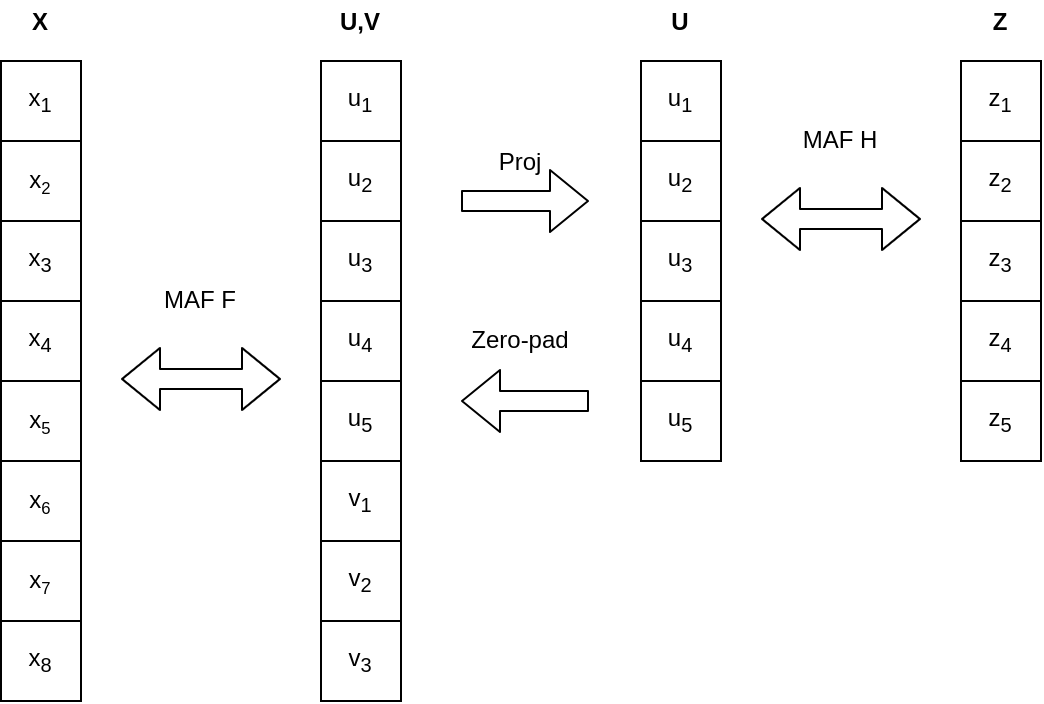
\includegraphics[width=0.7\textwidth]{img/mflow.png}
    \caption{An  example representation of dependencies between the data $\mathbf{x}$, latent variables $\mathbf{u}$, $\mathbf{v}$ and the normally distributed variable $\mathbf{z}$. Here the example data has 8 dimensions and the latent space has 5 dimensions. The bijective transformations are learned with Masked Autoregressive Flows (MAFs).}
    \label{fig:fig1}
\end{figure}

The training of this model is split in two phases completed sequentially for every batch. Firstly, the parameters of $ \mathrm{f}$ are updated by minimizing reconstruction error from the projection onto the manifold (loss function in Eq.~\ref{eq:eq3}). The second phase of training consists in updating the parameters of $\mathrm{h}$ by minimizing the negative log likelihood from Eq.~\ref{eq:eq4}. 

\begin{equation}
    \mathcal{L}_{manifold} = \lvert \lvert x-g(g^{-1}(x)) \lvert \lvert ^2
    \label{eq:eq3}
\end{equation}

\begin{equation}
    \mathcal{L}_{density} = \log p_{u}(g^{-1}(x))
    \label{eq:eq4}
\end{equation}

Regarding the preprocessing steps, the LHC Olympics datasets have been clustered and the the following features have been selected for each of the two leading jets: $p_T$, $\eta$, $E$, $m$, $\tau_3/\tau_2$, $\tau_2/\tau_1$, where $\tau_n$ is the n-subjettiness. For these 12 features, the best performing manifold size was 8.

This model offers the possibility to calculate both the density on the manifold and the reconstruction error from the projection on the manifold. We tried to use both of those metrics in order construct a robust anomaly score as in Eq.~\ref{eq:eq5}. This metric performs the anomaly detection task better on the R\&D dataset that its components and better than a basic normalizing flow model trained on the same data, judging by the ROC curves in Fig.~\ref{fig:fig2}.

\begin{equation}
    \mathcal{R}_{exp}(x) = \frac{\lvert \lvert x-g(g^{-1}(x)) \lvert \lvert ^2}{1+p_{u}(g^{-1}(x))}
    \label{eq:eq5}
\end{equation}

While experimenting with this anomaly score, it became apparent that it generates a bias towards events with high dijet mass ($m_{jj}$). In order to decouple $ \mathcal{R}_{exp}$ from $m_{jj}$ we included the marginal likelihood of $m_{jj}$, that was modeled using Kernel Density Estimation (KDE), as a term into the anomaly score. The resulting metric, denoted ${R}_{m_{jj}}$, uses the ratio between the likelihood on the manifold and marginal $m_{jj}$ likelihood as in Eq.~\ref{eq:eq6}.

\begin{equation}
    \mathcal{R}_{m_{jj}}(x) = \frac{\lvert \lvert x-g(g^{-1}(x)) \lvert \lvert ^2}{1+\frac{p_{u}(g^{-1}(x))}{p_{KDE}(m^{x}_{jj})}}
    \label{eq:eq6}
\end{equation}

Translating the performance obtained on the R\&D data to the black boxes proved to be a big challenge. The small differences in modeling from a black box to another are often enough to introduce significant biases. The only apparent solution seems to be training and applying the method on the same dataset.
%\noindent \textit{Please introduce the motivation for your method (not anomaly detection in general), how it works, and how you have implemented it.  Please include details about how you trained your algorithms and how you picked your hyperparameters.}

\subsection{Results on LHC Olympics}
\label{sec:results}

The R\&D dataset was heavily used for benchmarking different approaches, Fig.~\ref{fig:fig2} shows the anomaly detection performance of different metrics on the R\&D dataset. 

\begin{figure}[h!]
    \centering
    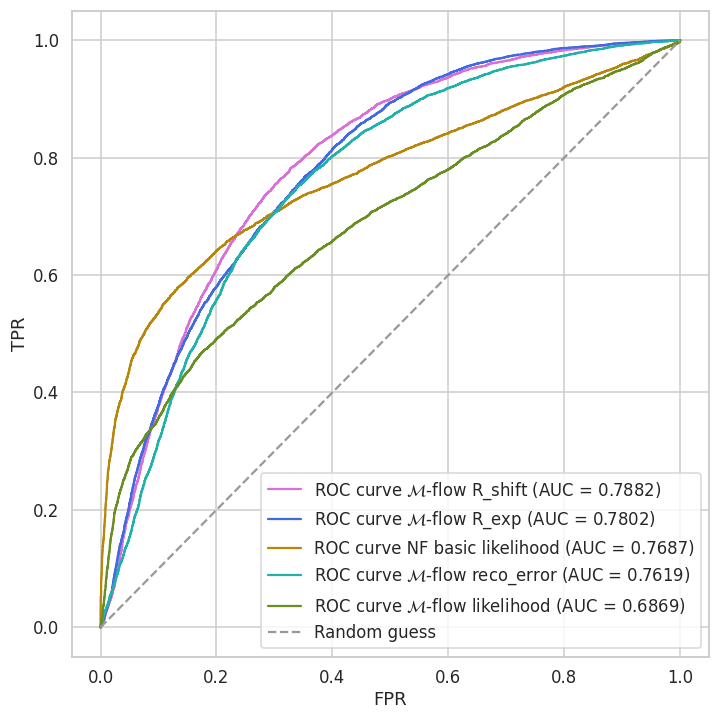
\includegraphics[width=0.5\textwidth]{img/mf_roc_all.png}
    \caption{Signal detection ROC curves in the R\&D dataset for different anomaly scores}
    \label{fig:fig2}
\end{figure}

In order to evaluate the performance of this method in the absence of pure background training data, a small fraction ($\sim 1\%$) of signal was introduced into a subsample from the R\&D dataset. The resulting data sample was used both for training and evaluation of the model.

Several cuts have been applied on $\mathcal{R}_{m_{jj}}$ while trying to find any indication of a resonance in the $m_{jj}$ spectrum. Although less apparent, there is still a bias towards identifying higher $m_{jj}$ events as being anomalous. The right plot in Fig.~\ref{fig:fig3} shows the $m_{jj}$ distribution for events above the $50^{th}$ percentile of $\mathcal{R}_{m_{jj}}$ vs events above the $70^{th}$ percentile of $\mathcal{R}_{m_{jj}}$. If we were to take the $50^{th}$ cut as a baseline, it is clear that increasing the threshold has the effect of selecting events with slightly higher $m_{jj}$. Unfortunately there is no sharp peak in the $m_{jj}$ distribution that would indicate a possible resonance, but rather the tail of the distribution seems to get bigger.

\begin{figure}[h!]
    \centering
    \begin{minipage}[b]{.5\textwidth}
        \centering
        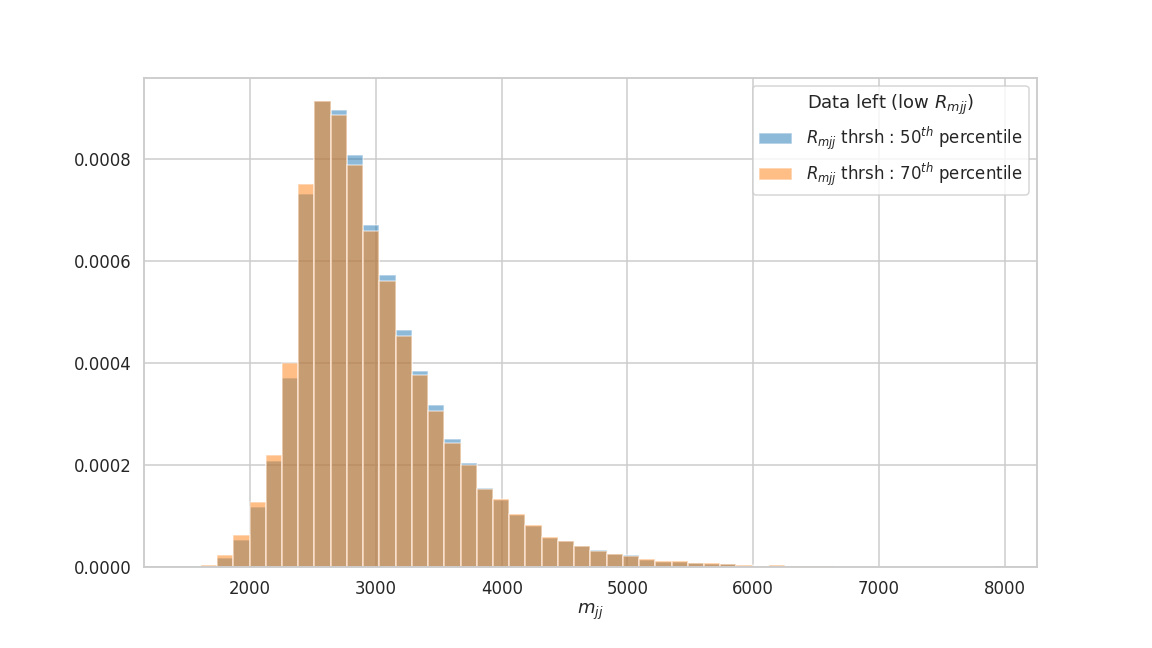
\includegraphics[width=\textwidth]{img/LLR_right.png}
        %\caption{$m_{jj}$ distribution of  below }
        %\label{fig:fig3}
    \end{minipage}%
    \begin{minipage}[b]{.5\textwidth}
        \centering
        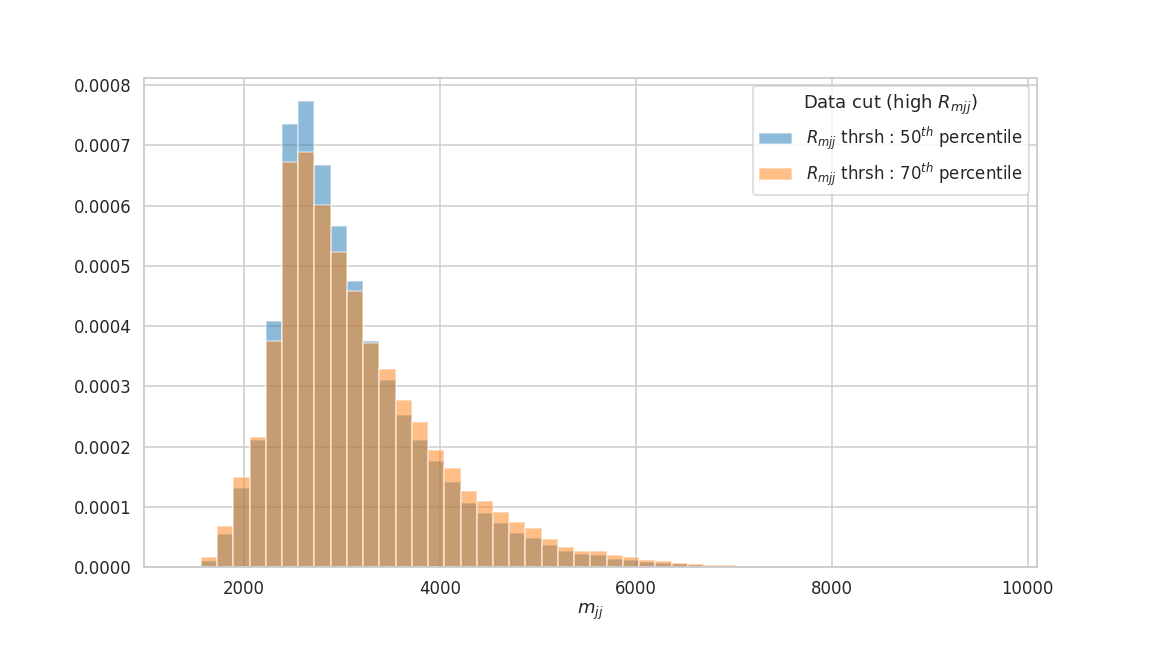
\includegraphics[width=\textwidth]{img/LLR_left.png}
        %\caption{Another figure}
        %\label{fig:fig4}
    \end{minipage}
    \label{fig:fig3}
    \caption{Overlapping $m_{jj}$ distributions below (left) and above (right) two threshold cuts on $\mathcal{R}_{m_{jj}}$. Distributions for a $50^{th}$ percentile cut are in blue, while  distributions for a $70^{th}$ percentile cut are in orange. The $x$ axis is in $GeV/c^2$.}
\end{figure}

The results so far suggest that this method can not be used reliably to find the hidden signal within the black-boxes. This behavior is consistent regardless of the choice of $\mathcal{R}_{m_{jj}}$ thresholds.
% \noindent \textit{We welcome results on any of the black boxes (BBs) as well as the R\&D dataset.  Please try to minimize any discussion of non-LHCO results.  Figures should be referenced like this: Fig.~\ref{fig:fig1}.}

% \begin{figure}[h!]
% \centering
% \includegraphics[width=0.5\textwidth]{RvslogPbg.pdf}
% \caption{Description of the figure.  Reproduced from Ref.~\cite{Nachman:2020lpy}.}
% \label{fig:fig1}
% \end{figure}

\subsection{Lessons Learned}
\label{sec:lessons}

One of the main lessons learned during this challenge is that: in absence of a good background model, the neural networks by themselves can not achieve good anomaly detection performance. 

For the winter LHC Olympics, we approached the problem with a simple autoencoder that was trained on the full background black box. Applying that model on Black Box 1 (BB1) introduced a lot of bias that ended up acting like a fake signal. Special precautions should always be taken in order to avoid this scenario.

With the experience gained from studying BB1 we were a lot more careful to avoid creating fake signal. The subsequent problem proved to be the lack of a good background model. Since we could not relay on the full background black box, the alternative was to train on data, but this comes with its own issues. 

All of the attempts so far came short of providing a good background modeling and therefore the current anomaly detection performance leaves a lot to be desired. Those trials taught us that a good machine learning anomaly detection algorithm is not just about the neural network itself, but many other analysis details should be treated with the same amount of attention.


% \noindent \textit{Please say anything that you learned from the experience in general, what you learned specifically from the results, what you improved after you learned about BB1, what you would change in the future, etc.}

\subsection{Code Availability}
\label{code:code}

Most of the machine learning heavy lifting was done with the help of the existing code base from the original $\mathcal{M}$-flow model introduced in Ref.~\cite{Brehmer:2020vwc} by Johann Brehmer and Kyle Cranmer. \href{https://github.com/johannbrehmer/manifold-flow}{https://github.com/johannbrehmer/manifold-flow} 
% \noindent \textit{Please consider sharing a link to your code!  All of the sample links will be included in the paper so no need to add those.}

%%%%%%%%%%%%%%%%%%%%%%%%
\acknowledgments

This work was supported by the U.S.~Department of Energy, Office of Science under contract DE-AC02-05CH11231. 

\vspace{10mm}

% \noindent \textit{For the references, please use names from Ref.~\cite{hepmllivingreview}.  If your paper is not there or is not updated, please submit a MR!}

\bibliographystyle{jhep}
\bibliography{HEPML}
\end{document}
